\documentclass[conference]{IEEEtran}
\IEEEoverridecommandlockouts
% The preceding line is only needed to identify funding in the first footnote. If that is unneeded, please comment it out.
\usepackage{cite}
\usepackage{lipsum}
\usepackage{amsmath,amssymb,amsfonts}
\usepackage{algorithmic}
\usepackage{graphicx}
\usepackage{hyperref}
\usepackage{pdfpages}
\usepackage{gensymb}
\usepackage{textcomp}
\usepackage{xcolor}

\hypersetup{
    colorlinks=false, %set true if you want colored links
    linktoc=all,     %set to all if you want both sections and subsections linked
    linkcolor=blue,  %choose some color if you want links to stand out
}

\begin{document}
\bstctlcite{IEEEexample:BSTcontrol}

\title{Convolutional Neural Networks for Super High Momentum Spectrometer Optics Pattern Recognition
%\thanks{Identify applicable funding agency here. If none, delete this.}
}

\author{\IEEEauthorblockN{Zain Mothupi}
\IEEEauthorblockA{\textit{Department of Physics} \\
\textit{University of Warwick}\\
Coventry, England \\
mothupizain@gmail.com}
%\and
%\IEEEauthorblockN{2\textsuperscript{nd} Given Name Surname}
%\IEEEauthorblockA{\textit{dept. name of organization (of Aff.)} \\
%\textit{name of organization (of Aff.)}\\
%City, Country \\
%email address or ORCID}
%\and
%\IEEEauthorblockN{3\textsuperscript{rd} Given Name Surname}
%\IEEEauthorblockA{\textit{dept. name of organization (of Aff.)} \\
%\textit{name of organization (of Aff.)}\\
%City, Country \\
%email address or ORCID}
%\and
%\IEEEauthorblockN{4\textsuperscript{th} Given Name Surname}
%\IEEEauthorblockA{\textit{dept. name of organization (of Aff.)} \\
%\textit{name of organization (of Aff.)}\\
%City, Country \\
%email address or ORCID}
%\and
%\IEEEauthorblockN{5\textsuperscript{th} Given Name Surname}
%\IEEEauthorblockA{\textit{dept. name of organization (of Aff.)} \\
%\textit{name of organization (of Aff.)}\\
%City, Country \\
%email address or ORCID}
%\and
%\IEEEauthorblockN{6\textsuperscript{th} Given Name Surname}
%\IEEEauthorblockA{\textit{dept. name of organization (of Aff.)} \\
%\textit{name of organization (of Aff.)}\\
%City, Country \\
%email address or ORCID}
}



\maketitle

\begin{abstract}
Our Research focused on developing algorithms for the recognition and prediction of specific tune patterns in spectrometer optics data from Experimantal Hall C at Jefferson Laboratory. The main goal was to create a machine learning model capable of recognizing optics patterns that would otherwise be tedious for humans to classify, in a mere matter of seconds with reasonably high accuracy. Specifically, we utilised the Keras deep learning Application Programming Interface(API) to build a Convolutional Neural Network(CNN). The CNN was trained on a dataset of 186 simulated optics patterns and a Cross-Entropy function was implemented to assess the model's accuracy throughout the training process. The model was able to reach an average accuracy close to 100\text{\%} and an average loss of approximately 0.3. The machine learning model's ability to predict output was then tested against a set of 60 new images and achieved an average accuracy of 83\text{\%}.  
\end{abstract}

%\begin{IEEEkeywords}
% Here you would put keywords that may be important to follow in the paper (maybe repeated terms of importance, e.g. neural networks, convolution, )
%\end{IEEEkeywords}

\section{Introduction}
Since the inception of Artificial Intelligence in the mid 20th century, there has been rapid progress towards the creation of systems capable of matching or even surpassing human ability. As a result, Machine Learning (ML) a subset of artificial intelligence, emerged. In ML computer systems learn to perform tasks without bein explicit instructions, they learn purely from a set of data. The concept of computers learning directly from data has led to many algorithms modelled after the way humans learn. In particular, Neural Networks were inspired by the wiring of the human brain, imitating the interconnectedness of the neurons.
 See Fig.\ref{fig:test_img}
\cite{NNPart1_VZ_2019}

% Here you would insert an image (for example, the cartoon of the neural network brain)
\begin{figure}[h]  % you can google what eahc of these options, e.g. [h!] means when placing a picture, and you can adjust accordingly
  \centering
  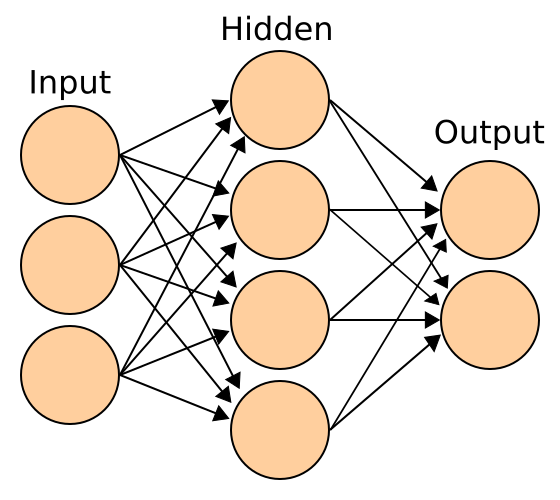
\includegraphics[scale=0.2]{images/Artificial_neural_network.png}
  \caption{Example of a figure caption.}
  \label{fig:test_img}
\end{figure}

In our research, we used a specific type of Neural Network known as a Convolutional Neural Network to interpret and analyse imgaes. All CNNs follow a basic list of steps in order to learn patterns from data.
\begin{itemize}
\item Receive input data
\item Make a prediction
\item Assess the prediction by comparing it to the desired output
\item Adjust its internal structure to give more accurate predictions the next time
\end{itemize}

A simple illustration of neural network architecture is shown in Fig. 2 (Give reference of picture here.)
\begin{figure}[h]
 \centering
  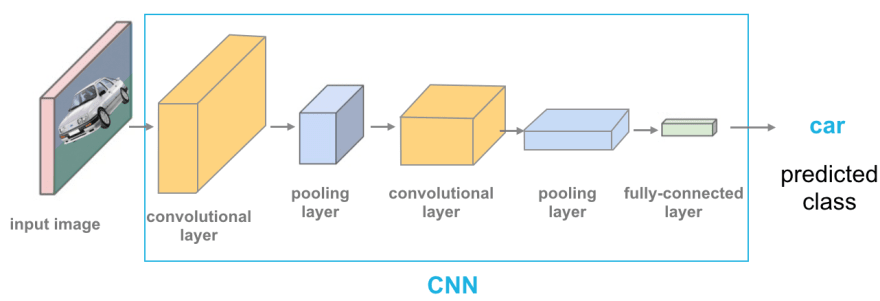
\includegraphics[scale=0.2]{images/ConvolutionalNeuralNetwork.png}
  \caption{Example of a figure caption.}
  \label{fig:test_img}
\end{figure}



\section{Methodology}
In this research, we analyze a total of 185 distinct simulated optics patterns from the Super High Momentum Spectrometer (SHMS) at Hall C of Jefferson Lab.
There were six different optics correlations ( $x_{fp}$ vs. $y_{fp}$,  $x_{pfp}$ vs. $y_{pfp}$, $x_{fp}$ vs. $y_{pfp}$,  $x_{pfp}$ vs. $y_{fp}$, $x_{fp}$ vs. $x_{pfp}$ and  $y_{pfp}$ vs. $y_{fp}$ . Each pattern had 31 optics images with varying optics tunes [Q1, Q2, Q3], corresponding to the spectrometer quadrupole magnets, summarized in Table \ref{tab:tune_stpSize}:

\begin{table}[h]
	\begin{center}
		\begin{tabular}{llll} % left-aligned, number of l's represent number of headings
                  \hline
                  Quadrupole Magnet & Range & Stepsize \\
                  \hline\hline
	          $Q1$ & [min, max] & stp1  \\
                  $Q2$ & [min, max] & stp2  \\
                  $Q3$ & [min, max] & stp3  \\                       
                  \hline 
		\end{tabular}
	\end{center}
	\caption{Caption of table.}
	\label{tab:tune_stpSize}
\end{table}

Each of the six 2D SHMS optics pattern correlations were trained separately, using 31 different optics tunes
per correlation plot for a total of 186 images. The optics patters for testing the network consisted of only
varying Q2 from 0.945 to 1.055 in steps of 0.01, while keeping Q1 and Q3 tunes fixed at unity.
To test the neural network after it had been trained, a set of 10 images were used for each 2D optics correlation, where Q1 and Q3
tunes were kept fixed at unity while Q2 was varied from 0.955 to 1.055 in steps of 0.01 for a total of 10 Q2 tunes.\\

IMPORTANT: Keep explaining what you did, or how was the data collected (I CAN HELP WITH THIS SINCE I WROTE THE CODES TO EXTRACT THE DATA IMAGES)
(See paragraph below, where I expalined roughly what I actually did. You can write this part as it is, and then put a citation that you got this
information through me. For example:  [3] Private communication. C. Yero. August 2021. (see references.bib in the current directory for bibliography format)

\section{Data Analysis Procedure}


%This figure position may need to be changed and put someplace else in this file, depending on whether it shows up
%in the location you want in your pdf. (Let me know if you have any issues with the placement of this picture)
\begin{figure*}
  \centering
  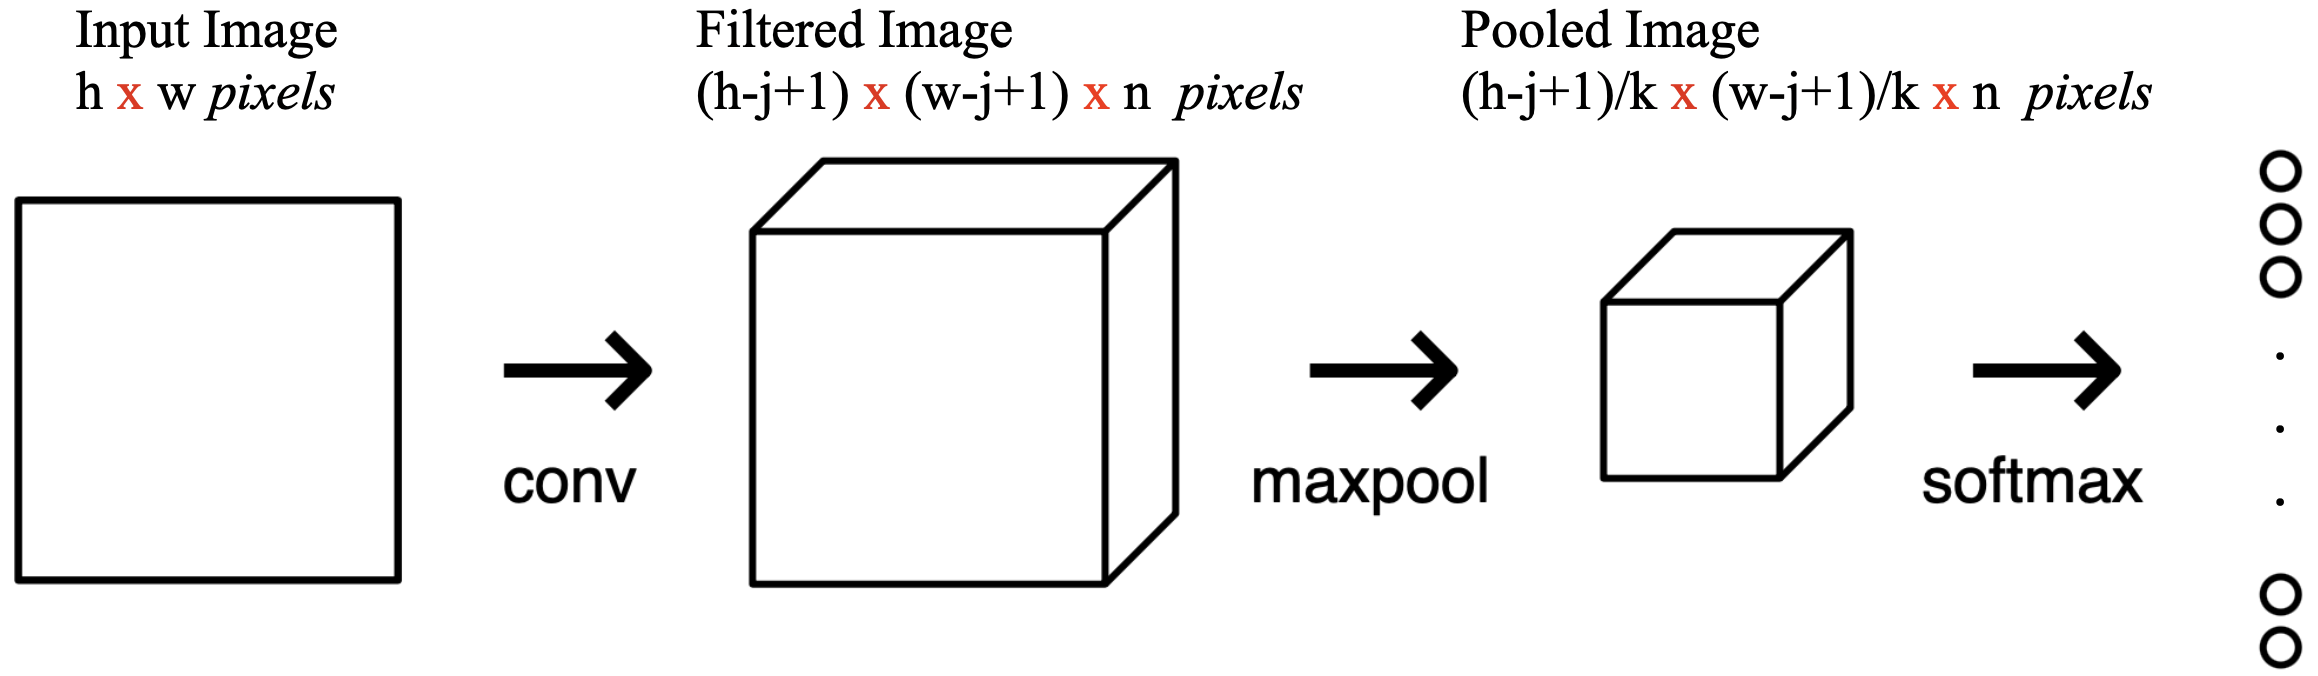
\includegraphics[scale=0.3]{images/CNN_layers.png}
  \caption{Description of image}
\end{figure*}
\indent Our Neural Network utilised 5 layers in total(See Fig.\ref{}). It consisted of input and output layers which represent the raw input image and output prediction and intermediate hidden layers each with a specific image analysis task. The intermediate layers are the Convolutional layer, Pooling layer and Activation layer described in the subsections below.\\
\subsection{Convolutional Layer}
The convolutional layer contains a set of 12 filters with dimension 6x6,  which are convolved with the input image and outputed by the layer. The process of convolving the image with the filters consists of overlaying the filter over s group of pixels(with the same dimensions as the filter), carrying out element-wise multiplication, calculating the sum of the results and using this as a pixel value in the output image. We then move on to the next possible grouping of pixels and continue the process until the entire image has been convolved with the filter. Convolutional layers help detect specific localized features in images which aids the model in making more accurate predictions.
, \cite{CNNPart1_VZ_2019}
\subsection{Pooling Layer}
We used a pooling size of 6 which decrease the size of  our input images from 200x200 to 32x32. This allows for the model to reduces the number of computations it has to perform while still preserving the important elements of the image. This is achieved by “pooling” or grouping pixel values together and selecting the maximum of the values which acts as a summary of the features present in the region, \cite{CNNPart1_VZ_2019}.
\subsection{Activation Layer}
The activation layer uses a function known as an activation function to transform an unbounded inout to a bounded output. In this research we used the Softmax function as our activation function. The Softmax function is given by the function $\text{Softmax}(x_{i}) = \frac{\exp(x_i)}{\sum_j \exp(x_j)}$ and turns the neural networks output values into probabilities which are more useful when evaluating our models predictions as it allows us to assess the certainty with which the NN makes a prediction. We assess our the performance of our NN using a loss function. The loss function compares the prediction of the NN to the actual value and calculates how far off the model is. This is then feed back to NN so that it can adjust its weights and biases to achieve a lower loss or higher accuracy (See Ref. \cite{}). For the layer description, give reference to the online blog you read, \cite{CNNPart1_VZ_2019}, and probably also
the article which describes what is softmax. You will need to probably add a new reference to the bibliography to be able to cite the softmax online article, similar to the other citations you have been doing.\\

The input image is passed through all the layers and the final output of the Softmax layer is a prediction. The prediction is then compared to the known result and the loss is calculated. A backpropagation method is used to minimize the loss by updating the parameters of the NN so as to decrease the loss. Each combination of a forward runthrough of  the NN and updating of parameters via backproagation is known as an epoch. The updated parameters are then analysed through the same process for a certain number of epochs so that the loss is minimized.
\indent The data with specific [Q1,Q2,Q3] tunes were simulated using the standard Hall C simulation program (\texttt{mc-single-arm})
and the raw data output was written to a ROOTfile. A separate ROOT C++ script (\texttt{make\_2Doptics.C}) was used to form each of
the six abovementioned 2D focal plane correlations correlations which were stored in a separate ROOTfile as histogram objects.
The 2D histograms were then converted to a 2D pixelated array and stored in binary format (.h5) via a Python code (\texttt{save2binary.py})
array to be read by the Neural Network using Python Keras. Each optics image used was 200x200 pixels and was passed thorugh each of
the hidden layers of the network described in Section 4 of this article.


\section{Results and Discussion}

\indent In our research our aim was to teach a computer to recognize optics patterns that would otherwise be tedious or difficult to distinguish for humans. Using the Keras API we trained and tested a CNN by providing simulated optics data from Jefferson Laboratory, Hall C. Each of the six 2D optics correlations were trained with 31 optics tunes and were able to reach and plateau at an accuracy of 98\% and a loss of 0.3 in 100 epochs. We used 10 test images per optics correlation and the network was able to correctly predict the patterns with at least 83\% accuracy. The results of the training are shown in Fig.\ref{}. These results prove that the computer can recognize these optics patterns with a reasonably high accuracy and as such can be used in support of humans to greatly reduce the time it takes to classify optics tune patterns.



\begin{figure*}
  \centering
  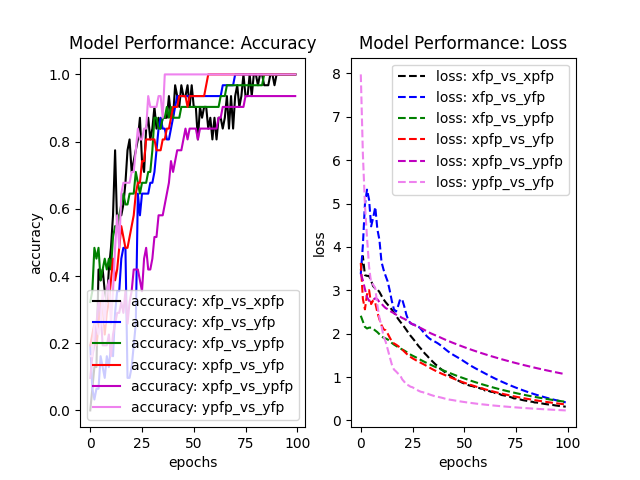
\includegraphics[scale=0.3]{images/Figure_1.png}
  \caption{Plot of Accuracy and Loss vs Number of Epochs}
\end{figure*}



The results of the test images is summarized in Table \ref{tab:results}
\begin{table}[h]
	\begin{center}
		\begin{tabular}{llll} % left-aligned, number of l's represent number of headings
                  \hline
                  col1 & col2 & col3 & col4 \\ \hline \hline
	          val1 & val2 & val3 & val4 \\
                  val5 & val6 & val7 & val8 \\
		  \hline 
		\end{tabular}
	\end{center}
	\caption{Caption of table.}
	\label{tab:results}
\end{table}

%dummy text
%\lipsum

\bibliography{references}   
\bibliographystyle{IEEEtran}



\end{document}
